\documentclass[12pt]{ltjsarticle}

\usepackage[T1]{fontenc}
\usepackage[utf8]{inputenc}
\usepackage[backend=biber, maxnames=100, backref=true]{biblatex}
\usepackage[binary-units = true]{siunitx}
\usepackage{amsmath, amssymb, amsthm}
\usepackage{graphicx}
\usepackage{hyperref}
\usepackage{ascmac}

\renewcommand{\thesection}{1.\arabic{section}}
\setcounter{section}{2}

\DeclareGraphicsRule{.ai}{pdf}{.ai}{}

\newcommand*{\exref}[1]{例~\ref{#1}}
\newcommand*{\fgref}[1]{図~\ref{#1}}

\newtheorem{example}{例}
\newtheorem{theorem}{定理}
\newtheorem{lemma}{補題}
\newtheorem{corollary}{系}

\addbibresource{reference.bib}

\begin{document}
\section{瞬時復号可能な符号}
瞬時復号可能な符号とは, 名前の通り, 符号がやってきたらそれを瞬時に復号可能な符号のことをいう.
これはつまり, 全てのメッセージを受信してから復号を行うのではなく, 来た時点で遅延なく復号可能な符号のことをいうのである.
厳密に言えば, 符号$\mathcal{C}$が\textbf{瞬時復号可能な符号}(instantaneously decodable code)あるいは\textbf{瞬時符号}(instantaneous code)であるとは,
各符号列$w_{i_1}, w_{i_2}, \cdots, w_{i_n}$に対し,
$\boldsymbol{t} = w_{i_1} w_{i_2} \cdots w_{i_n} \cdots$で始まる全ての符号列が
$\boldsymbol{s} = s_{i_1} s_{i_2} \cdots s_{i_n} \cdots$として一意に復号され,
その後に続く$\boldsymbol{t}$のシンボル列に無関係なことをいう.
\begin{example} \label{ex:not-uniquely}
  2元符号$\mathcal{C}$
  \begin{align*}
    s_1 \mapsto 0, s_2 \mapsto 10, s_3 \mapsto 11
  \end{align*}
  は瞬時復号可能な符号, つまり, メッセージ$\boldsymbol{t}$を受信しながら復号できる.
  なぜならば, $0$が来れば$s_1$に復号可能であるし, $1$が来れば, 次に来る符号を見てすぐに$s_2$なのか$s_3$なのかを判定できる.
\end{example}
\begin{example}
  2元符号$\mathcal{C}$
  \begin{align*}
    s_1 \mapsto 0, s_2 \mapsto 01, s_3 \mapsto 11
  \end{align*}
  は瞬時復号可能ではない.
  たとえば, $\boldsymbol{t} = 01111 \cdots$というメッセージが来たとき,
  $\boldsymbol{t} = 0.11.11.11. \cdots$なのか$\boldsymbol{t} = 01.11.11.11. \cdots$なのかはすぐには判定できず, メッセージ長が奇数か偶数かを見なければ判定することはできない.
\end{example}

一般に, 瞬時符号であれば一意復号可能な符号であることは成立するが, 逆は成立しない.
例えば, \exref{ex:not-uniquely}で定義する符号は一意復号可能だが, 既に見たように瞬時復号可能ではない.

符号$\mathcal{C}$が\textbf{語頭符号}(prefix code)であるとは, どの符号語$w_i$も他の符号$w_j \enspace (i \neq j)$の語頭にないことをいう.
すなわち
\begin{align*}
  \forall w \in T^*, w_j \neq w_i w
\end{align*}
である.
また, $C_1 = \emptyset$とも言い換えることもできる.
この語頭符号と瞬時符号との間には次のような関係がある.
\begin{screen}
  \begin{theorem}
    符号$\mathcal{C}$が瞬時符号であることと, 語頭符号であることは同値.
  \end{theorem}
\end{screen}
\begin{proof}
  まず, $\mathcal{C}$が瞬時符号であるとして, 語頭符号となることを示す.
  $\mathcal{C}$が語頭符号でないとする.
  このとき, ある$w_j$の語頭に$w_i$という符号列が含まれる.
  すると, $\boldsymbol{t} = w_i \cdots$で始まる符号列は$\boldsymbol{s} = s_i \cdots$にも,
  $\boldsymbol{s} = s_j \cdots$にも復号化される.
  よって, 符号$\mathcal{C}$は瞬時符号ではないが, $\mathcal{C}$が瞬時符号であることに矛盾.
  以上から, 符号$\mathcal{C}$は瞬時符号であれば, 語頭符号となる.

  次に, $\mathcal{C}$が語頭符号であれば, 瞬時符号でもあることを確認する.
  $\mathcal{C}$が語頭符号なので, $\boldsymbol{t} = w_i \cdots$であれば,
  この符号列は$\boldsymbol{s} = s_i \cdots$に復号化されなければならない.
  これは$w_i$は他の$w_j \enspace (i \neq j)$の語頭とはならないために, 一意に復号化されるためである.
  よって, どの符号列に対してもこの事実が成立するので,
  全てのシンボル列は$\boldsymbol{t}$の後続のシンボル列とは無関係となる.
  以上から, $\mathcal{C}$は瞬時符号となる.
\end{proof}

\section{瞬時符号の構成法}
$r$元瞬時符号は$r$分木によって構成することができる.
ここで考える$r$分木は\fgref{fg:r-ary-tree}のようにより根に空語$\epsilon$を配置し,
それに各シンボルを1つだけ加えたものを根の子にそれぞれ追加し,
以下同様にシンボルを1つずつ加えたものをそれぞれ子に...ということを繰り返す.
\begin{example}
  \label{ex:make-tree}
  語長を$4$までとしたときに構成される2分木は\fgref{fg:r-ary-tree}の通り.
  \begin{figure}
    \centering
    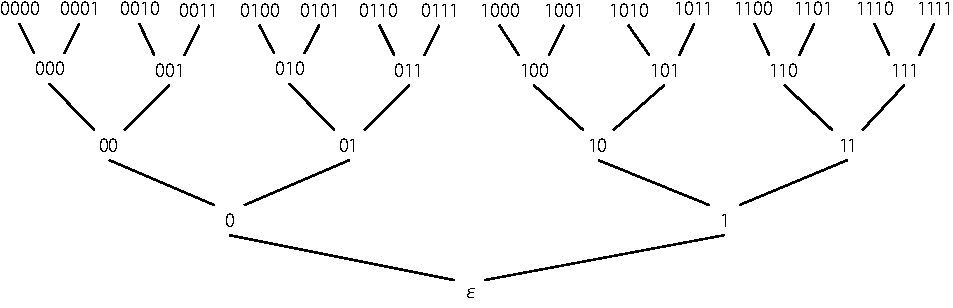
\includegraphics{image/2分木.pdf}
    \caption{語長$4$のときの2分木. 必ず根に近いノードの方をそのノード以降のノードは語頭として持っている.}
    \label{fg:r-ary-tree}
  \end{figure}
\end{example}

このようにして作った$r$分木に対して, 先程の語頭符号と瞬時符号が同値である命題を使い,
望む瞬時符号を構成していく.
まず, $r$分木のノードを1つ選ぶ.
次に, 選んだノード以降のノードを刈り込む(選んだノードの子や孫を削除する).
すなわち, 選んだノードを語頭に含んでいるノードを全て木から削除する.
これを繰り返すことで, 最終的に瞬時符号を構成することができる.
\begin{example}
  \exref{ex:make-tree}の中から$0, 10, 110, 1110, 1111$を符号語とした符号は瞬時符号となる.
  \fgref{fg:processed-r-ary-tree}の通り,
  選択したノードが必ず他の語を語頭とならないよう刈り込みがなされている.
  \begin{figure}
    \centering
    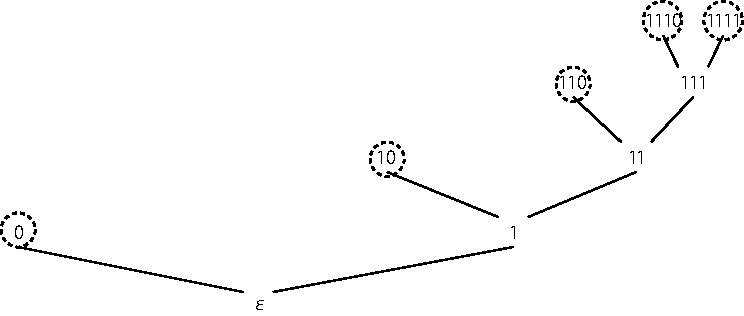
\includegraphics{image/構成された瞬時符号.pdf}
    \caption{\exref{ex:make-tree}からいくつか刈り込んで瞬時符号を構成している例. 符号として選ばれたノードは円で囲まれている.}
    \label{fg:processed-r-ary-tree}
  \end{figure}
\end{example}

\section{クラフトの不等式}
瞬時符号を$r$分木から構成するには, 除かれる葉の割合が$1$以下でなければならないという
当然の制限が存在する.
\begin{itembox}[l]{クラフトの不等式(Kraft's inequality)}
  \begin{theorem}
    符号長が$l_1, \cdots, l_q$であるような$r$元瞬時符号$\mathcal{C}$は,
    次の不等式を満たすとき, かつ, そのときのみ存在する.
    \begin{align*}
      \sum_{i = 1}^q \frac{1}{r^{l_i}} \leq 1
    \end{align*}
  \end{theorem}
\end{itembox}
\begin{proof}
  まず, 不等式を満たす符号が瞬時符号となることを示す.
  一般性を失うことなく, $l_1 \leq l_2 \leq \cdots \leq l_q$と仮定する.
  また, $l = \max \{l_1, \cdots, l_q\}$とし, $T^*$の高さ$l$までの部分を
  $T^{\leq l} = \bigcup_{i = 0}^l T^i$とする($T^i = \{w : |w| = i\}$).
  この集合から先程の$r$分木を作る手順で木をつくる.
  この木の高さ$l_1$において, ある符号$w_1$を$s_1$に割り当てることを考える.
  すると, その$w_1$を語頭に持つ高さ$l_1 + 1$以上のノード, つまり,
  $w_1$を頂点とした部分木は刈り込まれる.
  $r$分木であることから刈り込まれる部分木の葉は$r^{l - l_1}$個ある.
  ここで, 不等式
  \begin{align*}
    \sum_{i = 1}^q \frac{1}{r^{l_i}} \leq 1
  \end{align*}
  の両辺に$r^l$をかけると,
  \begin{align*}
    \sum_{i = 1}^q r^{l - l_1} \leq r^l
  \end{align*}
  となる.
  $q > 1$に対し, 明らかに
  \begin{align*}
    \frac{1}{r^{l_1}} < \sum_{i = 1}^q \frac{1}{r^{l_i}} \iff r^{l - l_1} < \sum_{i = 1}^q r^{l - l_i}
  \end{align*}
  となる.
  従って,
  \begin{align*}
    r^{l - l_1} < \sum_{i = 1}^q r^{l - l_i} \leq r^l
  \end{align*}
  となる.
  この刈り込みを$k < q$となる$k$まで続けると,
  刈り込まれた葉の数は$\sum_{i = 1}^k r^{l - l_i}$となるが, これは
  \begin{align*}
    \sum_{i = 1}^k r^{l - l_i} < \sum_{i = 1}^q r^{l - l_i} \leq r^l
  \end{align*}
  を満たす.
  この不等式からまだ刈り込まれていない葉が存在することがわかるので,
  その葉に繋っている$w_{k + 1}$を選択することができる.
  これによって, $q$まで符号語を選択することができる.
  この過程を通して, 選択された符号語を語頭として持つものは全て刈り込んで次のステップに移っていることから,
  選ばれた符号語を持つ符号は語頭符号となる.
  よって, 不等式を満たす符号語は瞬時符号となることが示された.
  \begin{figure}
    \centering
    \includegraphics{image/クラフトの不等式の説明図.ai}
    \caption{$w_1$を頂点とする部分木は$r^{l - l_i}$枚の葉を持つ.}
  \end{figure}

  次に, 符号$\mathcal{C}$が瞬時符号であるとして不等式を満たすことを示す.
  $\mathcal{C}$は瞬時符号なため, 語頭符号となる.
  従って, $T^{\leq l}$の葉は$\mathcal{C}$に属する多くとも1つの符号しか語頭に持たない.
  $\mathcal{C}$に属する符号語$w_i$は$r^{l - l_i}$枚の葉の語頭となるので,
  $\sum_{i = 1}^q r^{l - l_i}$枚の葉が$\mathcal{C}$のいずれかの符号語を語頭に持つことになる.
  $T^{\leq l}$は$r^l$枚の葉を持つので, 不等式
  \begin{align*}
    \sum_{i = 1}^q r^{l - l_i} \leq r^l
  \end{align*}
  が成立する.
  この不等式の両辺を$r^l$で割れば示したかった不等式が導出される.
\end{proof}

\section{マクミランの不等式}
先のマクミランの不等式と同じような不等式が, 実は一意復号可能な符号に対しても成立する.
\begin{itembox}[l]{マクミランの不等式(McMillan's inequality)}
  \begin{theorem}
    符号長が$l_1, \cdots, l_q$な一意復号可能な$r$元符号$\mathcal{C}$は
    不等式:
    \begin{align*}
      \sum_{i = 1}^q \frac{1}{r^{l_i}} \leq 1
    \end{align*}
    を満たすとき, かつ, そのときのみ存在する.
  \end{theorem}
\end{itembox}
\begin{proof}
  不等式を満たすときには瞬時符号が存在するが, 瞬時符号は一意復号可能な符号となるため,
  一意復号可能な符号が存在する場合に, 不等式が成立することを示す.

  まず,
  \begin{itemize}
    \item $\displaystyle K = \sum_{i = 1}^q \frac{1}{r^{l_i}}$
    \item $L = \max\{l_1, \cdots, l_q\}$
    \item $l = \min\{\l_1, \cdots, l_q\}$
  \end{itemize}
  とする.
  ここで, $K^n$を考える.
  この$K^n$は$\prod_{j = 1}^n r^{-l_{i_j}}$という項の和で表される.
  さらに,
  \begin{align*}
    j = \sum_{j = 1}^n l_{i_j}
  \end{align*}
  とする.
  全ての$i$に対し, $l \leq l_i \leq L$なので, $ln \leq j \leq Ln$となるので,
  $N_{j, n}$を$j$の重複を許した表現の仕方の数とすれば,
  \begin{align*}
    K^n = \sum_{j = l n}^{L n} \frac{N_{j, n}}{r^j}
  \end{align*}
  と表すことができる.
  $N_{j, n}$は$n$個の符号列$w_{i_1}, \cdots, w_{i_n}$を長さが$j$となるよう列の個数と同じとなる.
  その列の各々は長さが$j$となる符号列$\boldsymbol{t} = w_{i_1} \cdots w_{i_n}$を決定するが,
  符号$\mathcal{C}$は一意復号可能であるため, 各$\boldsymbol{t}$の表現の仕方は1通りしかない.
  したがって, $N_{j, n}$は$\boldsymbol{t}$の個数に等しいか少なくなる.
  よって, $N_{j, n} \leq r^j$となる.
  $K^n$は$Ln - ln + 1$個の項$N_{j, n} / r^j \leq 1$の和なので, 任意の$n \geq 1$に対し,
  \begin{align*}
    K^n \leq Ln - ln + 1 = (L - l) n + 1
  \end{align*}
  となる.
  $K, l, L$は$n$とは独立なため, $K > 1$ならば, $K^n$は指数関数的に増大する.
  しかし, $n$に線形な式で抑えられているため, 指数関数的に増大することはない.
  よって, $K \leq 1$でなければならない.
  従って, $K$の定義を思い出せば, 望んでいた不等式を得ることができる.
\end{proof}

このマクミランの不等式とクラフトの不等式から, 次の系がすぐに導ける.
\begin{screen}
  \begin{corollary}
    符号長が$l_1, \cdots, l_q$の$r$元瞬時符号は, これらの符号長をもつ,
    一意復号可能な$r$元符号が存在するとき, かつ, そのときのみ存在する.
  \end{corollary}
\end{screen}
この系自体は同じ不等式を, 一意復号可能な符号の存在も瞬時復号可能な符号の存在も,
同じ不等式を満たさなければならず, また, 存在すれば, 同じ不等式が満たされることから
すぐに従うことがわかる.

\printbibliography[title=参考文献]
\end{document}
